\documentclass{article}
\usepackage{graphicx}
\usepackage{amsmath}
\usepackage{hyperref}
\usepackage{float} % For the H placement specifier
\usepackage[margin=0.75in]{geometry} % Reduced margins
\title{Scalable Pipeline Architecture for a Spotify Playlist Recommender System}
\author{Pablo Sánchez Orozco, Nicolás Every Alvarez, Alberto Arath Figueroa Salomon}
\date{\today}

\begin{document}
\maketitle

\begin{abstract}
We propose a scalable machine learning pipeline designed for a Spotify playlist recommender system. Leveraging over one million playlists, our end-to-end pipeline is structured to handle large-scale data ingestion, rigorous validation, efficient processing, iterative model training, and comprehensive analysis, followed by seamless deployment. The architecture emphasizes a model lifecycle approach, ensuring that even small baseline models can evolve by integrating advanced algorithms over time, thus enabling a robust and future-proof recommendation system.
\end{abstract}

\section{Introduction}
The growth in digital music consumption has underscored the need for sophisticated recommender systems that can efficiently process large volumes of data and provide personalized recommendations. This paper details the architecture of a scalable pipeline that serves as the backbone of a Spotify playlist recommender system. With a focus on modularity and lifecycle management, our approach not only meets current data processing demands but is also designed to seamlessly evolve with new algorithmic advances.

\section{Pipeline Architecture}
The proposed pipeline consists of the following key components:

\subsection{Data Ingestion}
\begin{itemize}
    \item \textbf{Objective:} Efficiently ingest and partition of our tracks and playlist data, we might need to use a distributed file storaged
    \item \textbf{Implementation:} The system could use distributed file storage (e.g., Google Cloud Storage or AWS S3) to manage over one million playlists. Data is ingested using parallel processing frameworks such as Apache Beam, and stored in optimized formats like TFRecords to enhance throughput and scalability.
\end{itemize}

\subsection{Data Validation}
\begin{itemize}
    \item \textbf{Objective:} Ensure the integrity and quality of ingested data.
    \item \textbf{Implementation:} Automated routines, powered by tools like TensorFlow Data Validation (TFDV), check for missing values, inconsistencies, and anomalies. Establishing a reliable data schema early in the pipeline is critical for downstream processes.
\end{itemize}

\subsection{Data Processing}
\begin{itemize}
    \item \textbf{Objective:} Apply standard techniques to enhance and clean our playlist data set
    \item \textbf{Implementation:} Usage of scalers and encoders to handle categorical variables.
\end{itemize}

\subsection{Model Training}
\begin{itemize}
    \item \textbf{Objective:} Train robust baseline models while allowing for the integration of more advanced algorithms.
    \item \textbf{Implementation:} The training component is modular, initially employing collaborative filtering or other baseline techniques. The architecture is designed to facilitate easy upgrades and experimentation with deep learning models, leveraging scalable cloud-based compute resources.
    \begin{figure}[H]
      \centering
      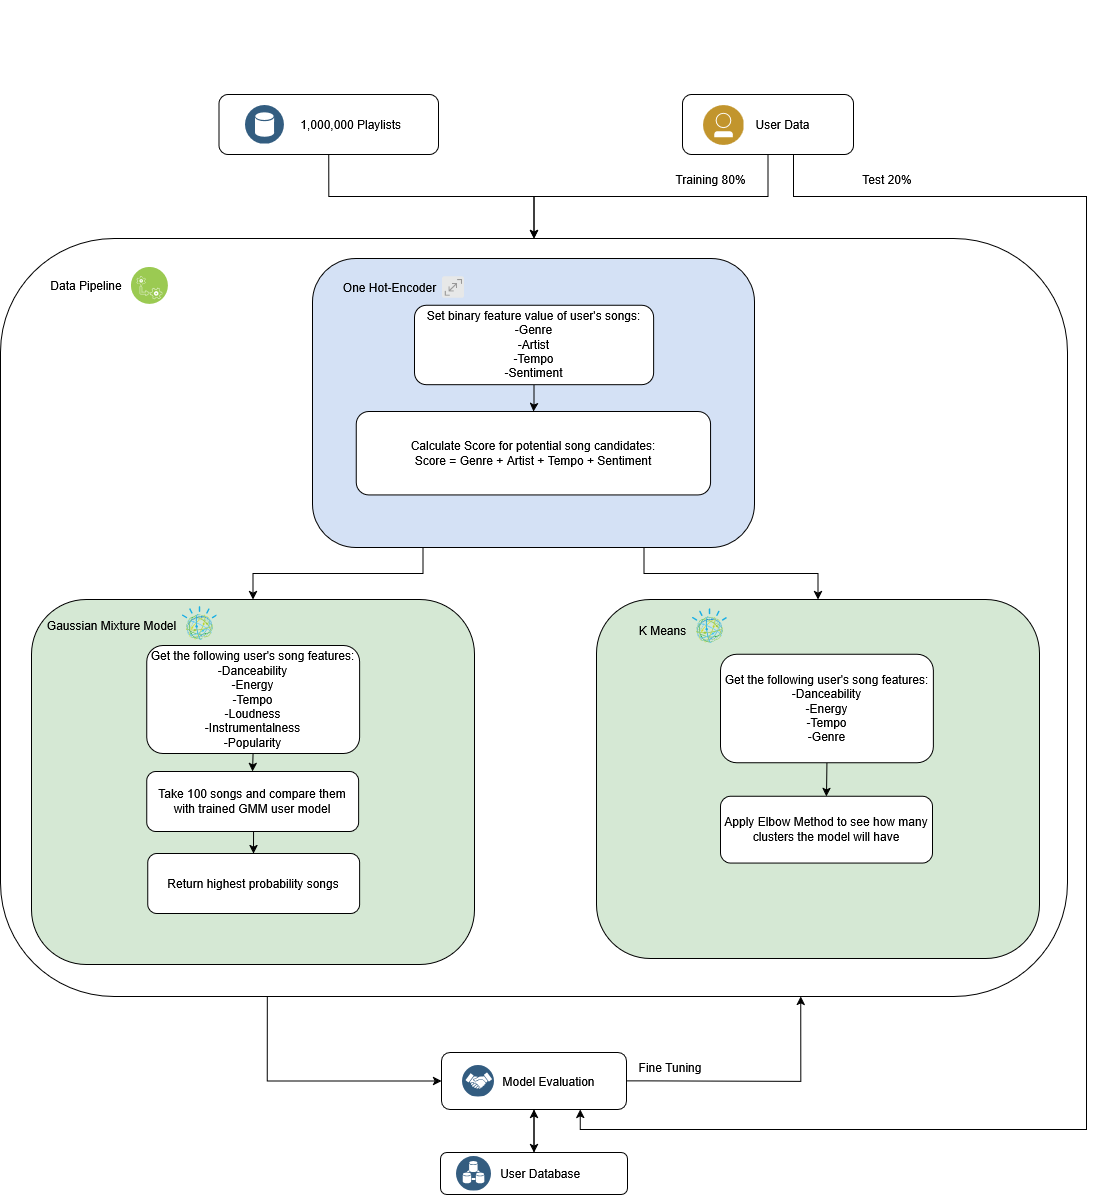
\includegraphics[width=0.8\textwidth]{Proyecto_Terminal.png}
      \caption{Project Terminal: Overview of the Model Training Workflow}
      \label{fig:project_terminal}
  \end{figure}
\end{itemize}

\subsection{Model Analysis and Validation}
\begin{itemize}
    \item \textbf{Objective:} Evaluate model performance and ensure high-quality recommendations.
    \item \textbf{Implementation:} 
    \begin{itemize}
        \item \textbf{User Content Splitting:} Since our training is unsupervised, we perform validation by splitting each user's content. A portion of the user's playlists or tracks is withheld during training.
        \item \textbf{Matching Recommendations:} The system then generates recommendations based on the trained model and compares these suggestions to the held-out selections from the same user.
        \item \textbf{Statistical Test Formulation:} We introduce a statistical test. The null hypothesis (\( H_0 \)) is that the recommendation system has no effect on user selections, while the alternative hypothesis (\( H_1 \)) is that the system improves alignment with user preferences. Based on the computed test statistic, we can use a t-test, chi-square test, or non-parametric tests (depending on the data distribution) to determine if the observed effect is statistically significant.
    \end{itemize}
\end{itemize}

\subsection{Model Deployment}
\begin{itemize}
    \item \textbf{Objective:} Deploy the trained model into production for real-time recommendations.
    \item \textbf{Implementation:} Deployment is managed via an automated CI/CD pipeline, which facilitates continuous integration and incremental updates with minimal downtime. This ensures the model lifecycle is maintained, allowing for regular updates and improvements.
\end{itemize}

\section{Scalability and Model Lifecycle Management}
\begin{itemize}
    \item \textbf{Modularity:} Each component (data ingestion, validation, processing, training, analysis, and deployment) design is decoupled as we are using a pipeline design, allowing independent updates and maintenance.
\end{itemize}

\section{Summary}
We have presented a comprehensive and scalable pipeline architecture for a Spotify playlist recommender system. By covering all critical stages—from data ingestion to model deployment—our design supports efficient handling of over one million playlists and is built with a model lifecycle approach to continuously evolve with advancements in recommendation algorithms. Future work will focus on integrating more sophisticated models and further optimizing each component of the pipeline for enhanced performance.


\end{document}